\section{Notation and Formal Setup}
\label{app:notation}

\paragraph{Observed data and policies.}
We observe i.i.d.\ logs
\[
O_i=(X_i,A_i,S_i,Y^{\mathrm{obs}}_i,L_i),\qquad i=1,\dots,n,
\]
generated under a fixed logger $A_i\sim \pzero(\cdot\mid X_i)$. A scalar judge
$S_i=s(X_i,A_i)$ is available on \emph{all} rows. The label indicator $L_i\in\{0,1\}$ marks inclusion in the oracle slice; when $L_i=1$ we observe $Y^{\mathrm{obs}}_i=Y_i$, otherwise $Y^{\mathrm{obs}}_i$ is missing.
For a candidate policy $\pprime$, define the sequence-level importance ratio
\[
W_{\pprime,i}
\;=\;
\frac{\pprime(A_i\mid X_i)}{\pzero(A_i\mid X_i)}
\;=\;
\exp\!\Big\{\log p_{\pprime}(A_i\!\mid\!X_i)-\log p_{\pzero}(A_i\!\mid\!X_i)\Big\},
\]
computed via teacher forcing (TF) with the model’s own tokenizer/rendering. Write
\[
W^{\mathrm{m1}}_{\pprime,i}
\;=\;
\frac{W_{\pprime,i}}{\tfrac{1}{n}\sum_{j=1}^n W_{\pprime,j}}
\]
for the sample–mean–one (SNIPS) baseline (global normalization over the evaluation cohort).

\paragraph{Estimand.}
Let $Y(\pprime)$ denote the outcome under the counterfactual draw $A\sim \pprime(\cdot\mid X)$.
The target is
\[
V(\pprime)=\E\!\big[Y(\pprime)\big].
\]

\subsection{Assumptions (compact)}
\label{app:assumptions}
\textbf{(D1) Fixed logger \& i.i.d.} $(X_i,A_i,S_i)$ are i.i.d.\ under $\pzero$; TF log-likelihoods are stable and well-defined.

\noindent\textbf{(D2) Overlap (positivity).} $\pzero(a\mid x)>0$ whenever $\pprime(a\mid x)>0$, and $\E_{\pzero}[W_{\pprime}^2]<\infty$.

\noindent\textbf{(D3) Judge coverage \& stability.} $S$ is well-defined under both $\pzero$ and $\pprime$; the Radon–Nikodym derivative on $\sigma(S)$ exists; the judge/rubric is stable on the analysis window.

\noindent\textbf{(J1) Oracle slice.} There exists an i.i.d.\ subsample $O=\{i:L_i=1\}$ with $m=|O|\ll n$ on which $Y$ is observed.

\noindent\textbf{(J2-M) Mean sufficiency (monotone).} $\E[Y\mid X,A,S]=\mu(S)$ with $\mu$ weakly nondecreasing. This structural assumption enables the EIF derivations (\cref{thm:sur-eif}); it is \emph{sufficient} for transport (T1) but not required when transport is verified via audit.\quad
\textbf{(J2-SI) Single-index fallback.} There exist $g^\star:\mathcal{S}\times\mathcal{X}\!\to\!\R$ and nondecreasing $\mu^\star$ such that $\E[Y\mid X,A,S]=\mu^\star\!\big(g^\star(S,X)\big)$. When $g^\star$ depends only on $S$, this reduces to J2-M; when covariates $X$ (e.g., response length) are included in $g$, the target remains $V(\pi')$ and the estimand is preserved provided the index is consistently estimated.

\noindent\textbf{(T1) Transport.} $\E_{\pi'}[Y - f(S,X)] = 0$. Calibration learned under $\pi_0$ is mean-unbiased under $\pi'$. This is the \emph{fundamental requirement} for valid surrogate-only policy value estimation. With an audit slice under $\pi'$, T1 is testable (\cref{prop:mean-transport}); without audit, T1 must be assumed (e.g., via J2-M/J2-SI or domain knowledge). See the assumption hierarchy in \cref{app:assumptions-ledger}.

\noindent\textbf{(R1) Tails/moments.} $\E[Y^2]<\infty$, $\E[S^2]<\infty$, and $\E_{\pzero}[W_{\pprime}^2]<\infty$. Under the exact $\mathrm{IsoMeanOne}_S$ projection with relative variance bound $\rho\ge1$, $\Var_n(\hat W_{\pprime})\le \rho\,\Var_n(W^{\mathrm{m1}}_{\pprime})$ (i.e., variance at most $\rho$ times the SNIPS baseline).

\noindent\textbf{(R2) Calibration consistency.} Reward calibration satisfies $\|\hat f(Z)-\E[Y\mid Z]\|_{L^2(P_Z)}=o_p(1)$, where $Z=S$ in monotone mode and $Z=g(S,X)$ (learned index) in two-stage mode. Weight stabilization satisfies $\|\hat W_{\pprime}-m^\star_\rho\|_{L^2(P)}=o_p(1)$, where $m^\star_\rho$ is the $S$-monotone, mean-one, variance-capped projection of $W_{\pi'}$ (see \cref{app:projections}); when $\E[W_{\pi'}\mid S]$ is itself monotone and satisfies the variance constraint, $m^\star_\rho=\E[W_{\pi'}\mid S]$.

\noindent\textbf{(R3) One-of-two rates with cross-fitting.} With nuisances $\hat q(x,a)\approx \E[R\mid x,a]$ and $\hat W_{\pprime}$,
\[
\|\hat q-q^\star_R\|_{L^2(P)}\cdot \|\hat W_{\pprime}-m^\star\|_{L^2(P)} \;=\; o_p(n^{-1/2}),
\]
e.g., either factor is $o_p(n^{-1/4})$ with the other consistent.

\subsection{Cross-fitting and folds}
\label{app:folds}
Let $F:\{1,\dots,n\}\!\to\!\{1,\dots,K\}$ be a deterministic fold map (e.g., a hash of $x\_id$). For any learner $\mathcal{L}$,
train $\hat\eta^{(-k)}=\mathcal{L}$ on $\{i:F(i)\neq k\}$ and use out-of-fold predictions
$\hat\eta^{\mathrm{OOF}}_i=\hat\eta^{(-F(i))}(O_i)$ in influence-function (IF) calculations. The same folds are reused across reward calibration, weight stabilization, and DR nuisances.

\subsection{Projection operators used by \CJE}
\label{app:projections}
\textbf{Monotone cone.} $\mathcal{M}_\uparrow=\{f:\R\!\to\!\R \text{ nondecreasing}\}$. The isotonic projector (PAVA) $\Pi_{\mathcal{M}_\uparrow}$ enjoys:
(i) $L^2$ optimality; (ii) \emph{mean preservation} on the training sample; (iii) \emph{dispersion reduction} by majorization.

\noindent\textbf{Mean-one cone for weights.} For $w\in\R^n$ ordered by $S$, define the mean-one isotonic projection
\[
\mathrm{IsoMeanOne}_S(w)
\;=\;
\argmin_{u}\ \sum_i (u_i-w_i)^2
\quad\text{s.t.}\quad
u\in\mathcal{M}_\uparrow(S),\ \tfrac{1}{n}\sum_i u_i=1,
\]
where $\mathcal{M}_\uparrow(S)$ denotes vectors nondecreasing in the $S$-order. This preserves the sample mean and weakly reduces empirical variance; hence $\ESS$ weakly increases (deterministically, by majorization).

\noindent\textbf{Simplex hull.} For centered IF columns $\{\phi^{(e)}\}_{e\in\mathcal{E}}$, let $\Phi=[\phi^{(e)}]$ and $\Delta=\{\alpha:\alpha_e\ge0,\ \sum_e\alpha_e=1\}$. Influence-function stacking solves
$\min_{\alpha\in\Delta}\alpha^\top \hat\Sigma\,\alpha$ with $\hat\Sigma=(1/n)\Phi^\top\Phi+\lambda I$.

\subsection{Reward calibration and weight stabilization primitives}
\label{app:ops}
\textbf{Reward calibration.} On $O=\{i:L_i=1\}$, fit $R=\hat f(Z(S))$ via:
(i) \emph{two-stage} (recommended): $Z(S,X)=\mathrm{ECDF}\{g(S,X)\}$ with a spline $g$, or
(ii) \emph{monotone-only}: $Z(S)=S$ when covariates are unavailable.
Use OOF predictions $R^{\mathrm{OOF}}$ along IF paths; the point estimate may use a pooled fit. A terminal isotonic step enforces \emph{slice-mean preservation}.

\begin{figure}[t]
  \centering
  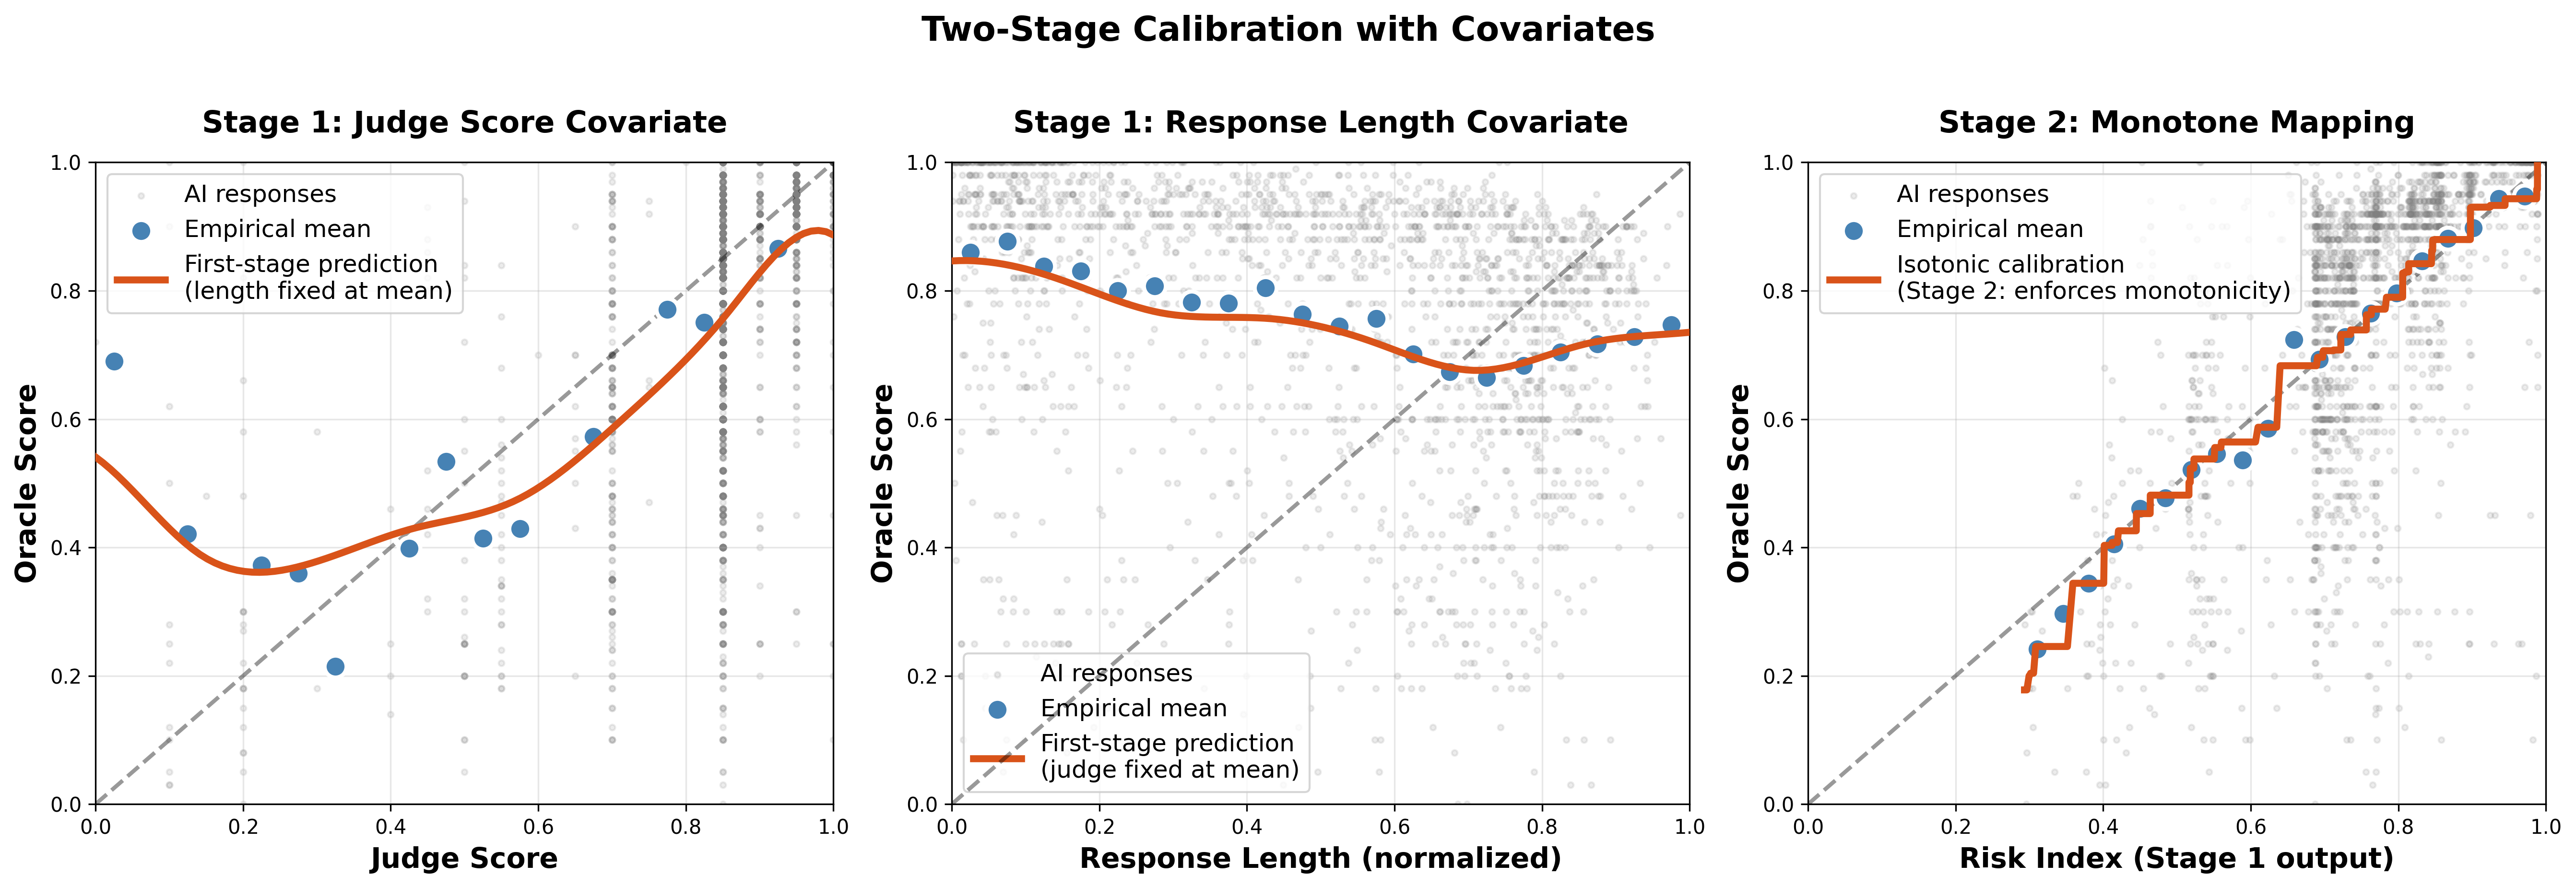
\includegraphics[width=\textwidth]{figs/two_stage_with_cov.png}
  \caption{\textbf{Two-stage calibration with covariates.} Left: first-stage spline on judge score (response length fixed at mean). Center: first-stage effect of response length (judge score fixed). Right: second-stage isotonic mapping on the risk index (Stage 1 output) enforces monotonicity while preserving flexibility from the first stage.}
  \label{fig:two-stage-detail}
\end{figure}

\noindent\textbf{Weight stabilization.} (Per fold) Fit up/down isotonic maps on $S$ to obtain $W^{\mathrm{OOF}}_{\uparrow},W^{\mathrm{OOF}}_{\downarrow}$; optionally include $W^{\mathrm{OOF}}_{\mathrm{base}}\equiv 1$. Define residuals $\Delta_i$ (IPS: $R_i$; DR: $R_i-\hat q(X_i,A_i)$). Choose
$\hat\beta\in\arg\min_{\beta\in\Delta_3}\beta^\top \hat\Sigma\,\beta$ where $\hat\Sigma$ is the covariance of $U_c=W^{\mathrm{OOF}}_c \Delta$. Form $W^{\mathrm{stack}}=\sum_c \hat\beta_c W^{\mathrm{OOF}}_c$, renormalize to mean one (global, over the evaluation cohort), optionally apply the \emph{absolute variance guard}
\[
\alpha=\min\!\Big\{1,\ \sqrt{\frac{\rho}{\Var(W^{\mathrm{stack}})}}\Big\},\qquad
W^{\mathrm{blend}}=1+\alpha\,(W^{\mathrm{stack}}-1),
\]
and normalize to mean one: $\hat W_{\pprime}=W^{\mathrm{blend}}/\bar W^{\mathrm{blend}}$. (The theoretical Lemma~\ref{lem:guard} uses a relative bound.)

\subsection{DR nuisances and sequence value}
\label{app:nuisances}
Let $\hat q(x,a)\approx \E[R\mid x,a]$ and define $\hat g_{\pprime}(x)=\sum_a \pprime(a\mid x)\,\hat q(x,a)$. For sequences, approximate $\hat g_{\pprime}(x)$ with one (default) rollout $A'\!\sim\!\pprime(\cdot\mid x)$ and $R'=\hat f\!\big(s(x,A')\big)$; a light smoother (e.g., ridge over $(x,z)$ features) can reduce Monte Carlo noise. Cross-fitting is used throughout.

\subsection{Influence functions and variance}
\label{app:if-var}
Let $\{\phi_i\}_{i=1}^n$ denote the (approximately) centered influence–function contributions of $\hat\psi$, computed with cross–fitted/OOF nuisances and $R^{\mathrm{OOF}}$ along the IF path, so that $\frac{1}{n}\sum_{i=1}^n \phi_i \approx 0$. Under standard regularity conditions,
\[
\sqrt{n}\,\bigl(\hat\psi-\psi\bigr)\ \overset{d}{\longrightarrow}\ \mathcal{N}\!\left(0,\ \Var(\phi)\right),
\quad\text{hence}\quad
\Var(\hat\psi) \approx \frac{\Var(\phi)}{n}.
\]
Since $\E[\phi]=0$, we have $\Var(\phi)\approx \frac{1}{n}\sum_{i=1}^n \phi_i^2$. We estimate the variance of $\hat\psi$ (not $\phi$) and the total variance (including the oracle addition) by
\[
\widehat{\Var}_{\mathrm{main}}
\;=\;
\frac{1}{n^2}\sum_{i=1}^n \phi_i^2,
\qquad
\widehat{\Var}_{\mathrm{total}}
\;=\;
\widehat{\Var}_{\mathrm{main}}+\widehat{\Var}_{\mathrm{cal}},
\]
and report the $(1-\alpha)$ Wald interval
\[
\CI_{1-\alpha}:\ \hat\psi \ \pm\ z_{1-\alpha/2}\,\sqrt{\widehat{\Var}_{\mathrm{total}}}\,.
\]
When serial or cluster dependence is a concern, we additionally report dependence–robust SEs (e.g., cluster–robust sandwich or block/stationary bootstrap) as a sensitivity analysis.


\subsection{Calibration-aware jackknife}
\label{app:oua}
Partition $O$ into $K$ oracle folds $\{O_k\}_{k=1}^K$. For each $k$, refit reward calibration on $O\setminus O_k$, recompute $R^{(-k)}$, and rerun the full pipeline to obtain $\hat\psi^{(-k)}$. Then
\[
\bar\psi=\tfrac{1}{K}\sum_{k=1}^K \hat\psi^{(-k)},
\qquad
\widehat{\Var}_{\mathrm{cal}}=\frac{K-1}{K}\sum_{k=1}^K \big(\hat\psi^{(-k)}-\bar\psi\big)^2.
\]
(With unequal fold sizes, use the standard \emph{weighted} delete-one-group formula.)

\subsection{Diagnostics (definitions)}
\label{app:diagnostics-defs}
\textbf{ESS.} $\ESS(W)=\big(\sum_i W_i\big)^2/\sum_i W_i^2$; we report the fraction $\ESS/n$. Under global mean-one normalization (SNIPS), $\sum_i W_i=n$ and
\[
\frac{\ESS(W)}{n}\;=\;\frac{1}{1+\mathrm{CV}^2(W)}\quad\text{with}\quad \mathrm{CV}^2(W)=\Var(W)\ \text{(since }\E[W]=1\text{)}.
\]
Unless stated otherwise, diagnostics use the global (not per-fold) mean-one scaling.

\noindent\textbf{Max-weight share.} $\max_i W_i\big/\sum_j W_j$.

\noindent\textbf{Tail index (Hill).} For top-$k$ order statistics $W_{(1)}\ge\cdots\ge W_{(k)}$,
$\hat\alpha^{-1}=\tfrac{1}{k}\sum_{j=1}^k \log\!\big(W_{(j)}/W_{(k)}\big)$ (we sweep $k$ over a stability grid and report the plateau).

\noindent\textbf{Bhattacharyya affinity in $S$.} $A_B=\int \sqrt{p_{S|\pprime}(s)\,p_{S|\pzero}(s)}\,ds$ (discrete: sum over bins); $D_B=-\log A_B$.

\noindent\textbf{DR orthogonality score.} $n^{-1}\sum_i \hat W_{\pprime,i}\big(R^{\mathrm{OOF}}_i-\hat q^{\mathrm{OOF}}(X_i,A_i)\big)$ with a Wald CI.

\noindent\textbf{Coverage badge.} Plug-in estimate of $\Pr_{\pprime}\!\big(S\notin [S_{\min}^{\mathrm{orc}},S_{\max}^{\mathrm{orc}}]\big)$; large out-of-range mass with near-flat boundaries triggers \textsc{Limited Calibration Support} and \RefuseLevel.

\subsection{Symbol glossary}
\label{app:glossary}
\begin{center}
\begin{tabular}{ll}
\toprule
Symbol & Meaning \\
\midrule
$X,A$ & Context, action (sequence) \\
$S=s(X,A)$ & Judge score (scalar) \\
$Y$ & Ground-truth outcome (on oracle slice) \\
$\pzero,\pprime$ & Logger and candidate policies \\
$W_{\pprime}$ & Importance ratio $\pprime(A\mid X)/\pzero(A\mid X)$ \\
$W^{\mathrm{m1}}_{\pprime}$ & Mean-one (SNIPS) baseline \\
$R=\hat f(Z(S))$ & Calibrated reward (monotone or two-stage) \\
$\hat W_{\pprime}$ & Stabilized, unit-mean, $S$-monotone weights \\
$\hat q,\ \hat g_{\pprime}$ & Outcome and policy–value nuisances for DR \\
$\phi$ & Per-row centered influence-function contribution \\
$\widehat{\Var}_{\mathrm{main}}$ & Estimator variance $n^{-2}\sum_i\phi_i^2$ \\
$\widehat{\Var}_{\mathrm{cal}}$ & Calibration variance (oracle jackknife) \\
$\ESS(W)$ & Effective sample size \\
\bottomrule
\end{tabular}
\end{center}
